\chapter{Middle-level Intermediate Representation}

This chapter describes SableWasm's middle-level intermediate representation (MIR), which has a critical role in the entire compilation pipeline. MIR acts as a middle ground between the WebAssembly bytecode frontend and various possible backend. SableWasm only implements one backend that currently utilizes the LLVM compilation framework, but adding more backend support should not require significant modification on the MIR. It also implements an analysis and transformation framework where we perform several optimizations over the MIR. We will first go over the overall design of the MIR, then later move to the translation strategy we used to translate WebAssembly bytecode to MIR. Finally, we will end the chapter with several analyses and transformations we implemented.

\section{MIR Design}

In the previous chapters, we have quickly covered the design of WebAssembly bytecode. A quick reminder, WebAssembly is a stack-based intermediate representation (IR) where all instructions operate over an implicitly declared operand stack. There are several advantages of stack-based IR. Perhaps the most important one is its portability. A stack-based IR makes fewer assumptions on the machine than a register-based one.  One can even provide an implementation for a hypothetical machine with only one register. Another advantage is the code size. Experiments show that, in general, stack-based IR is relatively more minor in size than its corresponding registered version \cite{stack-and-register-vm}. When designing a binary format that ships executables over the internet, the stack-based IR seems to be a better choice for WebAssembly.

Nevertheless, there are no silver bullets; stack-based IR design has its drawbacks. One of them is the difficulty when performing code analysis and transformation over the module. As for each instruction, its operands implicitly come from the stack; the value use-def relationship between instructions is not apparent to the analysis, and recover such connection between instructions from the IR is not a trivial task.

\begin{figure}
  \centering
  \lstinputlisting[language=SableWasmMIR, basicstyle=\small\ttfamily, numbers=left]
  {Code/4.MIR/fibonacci.mir}
  \caption{Fibonacci in translated SableWasm MIR}
  \label{fig:mir-fibonacci}
\end{figure}

On the other hand, we have the register-based intermediate representation, more specifically, the infinite-register machine. The infinite-register machine is similar to what one would expect from an actual physical machine. The only difference that the infinite-register machine, as the name suggests, has an infinite amount of registers. For each instruction in register-based IR, it has its operand encoded in the instruction. Hence, the use-definition relationship will become explicit to the analysis and transformation. The main design goal for SableWasm MIR is to provide an analysis platform for the entire compiler system. Thus, we implement our MIR as an infinite register machine. We also take a traditional approach in various other aspects. For example, instead of using the structured control flow similar to what WebAssembly offers, we use control-flow graphs (CFGs) to represent the relationship between basic blocks. The SableWasm MIR is also in single static assign (SSA) form \cite{ibm-ssa}, covered in the background chapter. The design for instruction and module-level entities in SableWasm MIR is quite similar to what WebAssembly instruction offers. One can view the SableWasm MIR as a mixture of LLVM intermediate representation and WebAssembly bytecode. We also adopt several design features from LLVM IR into MIR, such as use site lists. In SableWasm MIR, all elements are derived from the base class \texttt{ASTNode} which offers the implementation to these features. The base class automatically manages the use sites list, which is helpful later in MIR analysis and transformation.

Figure~\ref{fig:mir-fibonacci} shows a simple function that calculates Fibonacci numbers with a recursive method in SableWasm. With the help of the figure, we will go through the detailed design of SableWasm later in the chapter. We will first present the module-level entity design and their initializer expressions, such as functions, then move to the design of each instruction defined in MIR.

\subsection{MIR Initializer Expressions}

\begin{figure}
  \centering
  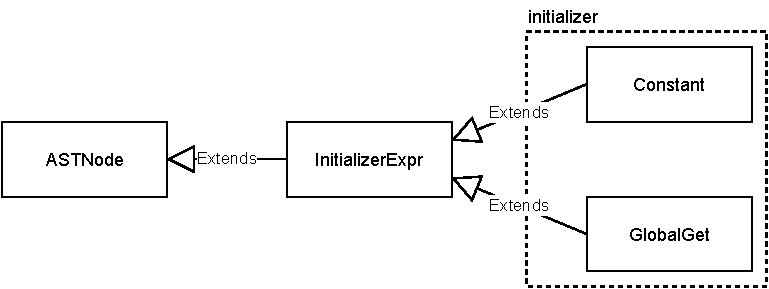
\includegraphics[width=\textwidth]{Images/4.MIR/initalizer-expression.pdf}
  \caption{SableWasm MIR Initializer Expression}
  \label{fig:sablewasm-mir-initializer-expression}
\end{figure}
   
WebAssembly defines a particular form of expression, namely constant expressions. They can appear in three locations in the current specification. First, global variables declaration can contain constant expression as their initialization values. Additionally, data section entries and element section entries can have constant expressions as the offsets for their initialization payload. In SableWasm MIR, we define initializer expressions that act similar to what constant expression does in WebAssembly. Figure~\ref{fig:sablewasm-mir-initializer-expression} gives a general illustration about SableWasm MIR initializer expressions. The initializer expressions are quite simple. In the current WebAssembly and SableWasm, an initializer expression can be either a constant value or refer to an imported global via \texttt{GlobalGet} instruction. Hence, in principle, currently, SableWasm MIR initializer expression is essentially a single instruction. In the future, one may generalize such constrain by allowing more complex constructs in initializer expressions. 

\paragraph{Constant}
The \texttt{Constant} instruction represents a single constant value for the initializer expression. In WebAssembly, a constant value can be one of the following: a 32-bit or 64-bit integer, a floating-pointer number or a 128-bit SIMD vector \footnote{with WebAssembly SIMD128 extension}, and the specification encodes type within the instruction opcode. Hence, there are multiple instructions in WebAssembly to introduce a constant. In SableWasm, we do not encode the type into the opcode, and \texttt{Constant} instruction is the only instruction that takes care of the task. In figure~\ref{fig:sablewasm-mir-initializer-expression}, we have a constant initializer at line 6 that initializes the values of the global to a 32-bit integer with a value that equals 66560. When querying the type of a \texttt{Constant} instruction, SableWasm will infer it from its payload constant.

\paragraph{GlobalGet}
The \texttt{GlobalGet} instruction is exactly same as the WebAssembly's \texttt{global.get} in execution semantics. WebAssembly specification allows any initializer refers to an imported \footnote{This might subject to change in the future version of WebAssembly} global value. As these values are initialized before the module, reading the value from them is always valid during module initialization. The example in the figure does not provide an example of \texttt{GlobalGet} as an initializer expression. They are less frequently used compare to constant initializer expression, especially for global values. However, in some ABI implementations, data section entries and element section entries require to read from global values serving as base pointers. SableWasm also infer the type for \texttt{GlobalGet} initializer expression in a similar fashion as \texttt{Constant}. In this case, the type of instruction is the same as the referred global variable without the constness modifier.

In this section, we cover the design and implementation of initializer expressions in SableWasm. They are pretty simple in the current design. We will now move to the next part in the SableWasm design, the module-level entities.
\subsection{MIR Module Entities}

\begin{figure}
  \centering
  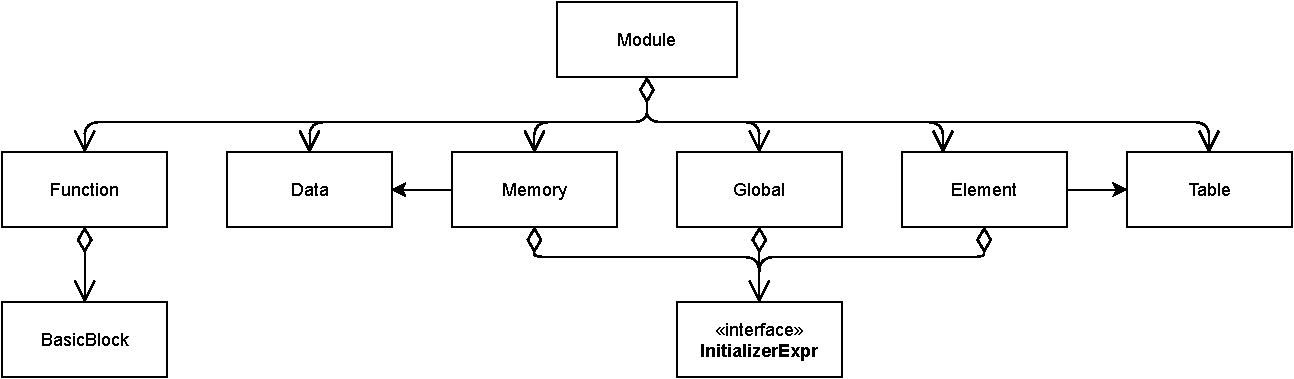
\includegraphics[width=\textwidth]{Images/4.MIR/module.pdf}
  \caption{SableWasm MIR Module-level entities}
  \label{fig:sablewasm-mir-module}
\end{figure}

SableWasm module-level entities are the top-level elements in a translation module. They are direct implements of the WebAssembly module entities defined in the specification. Figure~\ref{fig:sablewasm-mir-module} presents a general illustration of the SableWasm module-level entities. In this section, we will cover the design of each entity and compare them with its WebAssembly correspondent.

\paragraph{Function}
In figure~\ref{fig:mir-fibonacci}, we have a function definition at line 8. A function declaration in SableWasm provides information about the type, local variables and name. A function definition should satisfy all the requirements of function declaration, and additionally, provides a function body using basic blocks. The design of the function declaration and definition in SableWasm is quite similar to that of WebAssembly. The major difference is how to represent the function body. We will come back to this in the later sections within the chapter. Finally, like other module-level entities, a SableWasm function can optionally have import or export annotations. These annotations provide names for the import and export entries in the WebAssembly module.

\paragraph{Global}
SableWasm's global variable declaration and definition follow the design in WebAssembly. In SableWasm, we relax several of the constrain defined in WebAssembly specification and its extensions. In the SIMD extension proposal, the 128-bit vector type is only suitable within the function body. There is no direct way to pass a vector value to the host environment, as there is a lack of standard representation for 128-bit packed vectors in JavaScript \footnote{This might subject to change in the future. WebAssembly SIMD extension proposal is still in the drafting process.}. In  SableWasm, we treat all primitive types uniformly. Thus, a global variable can contain an integral value, a floating-point value or even a packed SIMD vector. The type for the global variable follows the specification in WebAssembly; it is a pair of value type and constness modifier. In figure~\ref{fig:mir-fibonacci}, we have a global definition at line 6, which contains a mutable 32-bit integral value. All global variable definitions in SableWasm must provide a value initialization via initializer expression, which we covered in the previous section. The rules for import and export annotation on the SableWasm function entities also apply to SableWasm global variables, which we do not show in the example above.

\paragraph{Memory and Data}
Memory and Data are implementation for WebAssembly linear memory and its initializer, respectively. One might think that there is no need to separate the memory initializer from the memory entity definition, as in WebAssembly specification, all data section entries must provide a valid linear memory index. In the early version of SableWasm, we indeed adopt such implementation. However, this approach might be subject to a significant change in an extension that might soon merge to the WebAssembly specification. The WebAssembly bulk memory operation extension proposal \footnote{WebAssembly bulk memory operations: \\\url{https://github.com/WebAssembly/bulk-memory-operations}} introduce new instructions, such as \texttt{memory.fill} that direct refers to a data section segment. Moreover, the proposal relaxes the constrain on the linear memory index. Now the index can behave like a flag indicating whether the data segment itself is active or not and no longer serves as a linear memory index. Hence, to make our framework `futureproof', we separate the linear memory declaration from their initializers. Figure~\ref{fig:mir-fibonacci} presents a linear memory definition at line 2. SableWasm memory entities also adopt WebAssembly linear memory type. The type consists of a pair of unsigned integers, indicating the lower bound and upper bound of the memory size in WebAssembly pages. Finally, the memory entity can have import and export annotations similar to other module-level entities in SableWasm. The example above defines a memory with a minimal size of 2 pages, 128KiB, and exports it under `memory'. The example above does not provide any example for data initializers, but they are quite easy to understand. A data initializer is essentially a binary chunk with an initialization offset. They are semantically equivalent to a data section entry in an ELF file.

\paragraph{Table and Element} SableWasm table and element entity implements the indirect table and its initializer, namely element segment, accordingly. They follow the simple principle as the memory and data entity in the previous section. Currently, like data segment entry, WebAssembly's element section entry must refer to a valid indirect table via an index. In the future, this may also subject to change. WebAssembly reference types extension proposal \footnote{WebAssembly reference types: \url{https://github.com/WebAssembly/reference-types}} introduce instructions such as \texttt{table.fill} that are able to have direct access to element segment initializers. \texttt{table.fill} instruction is similar to \texttt{memory.fill} defined in the bulk memory operation extension. It will copy a sequence of compile-time defined function pointers into an indirect table at runtime. Thus, when we design our table entity, we also split the declarations from their initializers. The type for table entity is the same as the table type in WebAssembly. It consists of a pair of unsigned integers, indicating the lower bound and upper bound for the number of function pointers stored in the indirect table. In SabelWasm MIR, we treat memory entities and table entities as black boxes, and its concrete implementation is deferred to the backend. The example shown in figure~\ref{fig:mir-fibonacci}, the module defines a table entity at line 4 that stores exactly one function pointers. Note that the table entity does not require users to initialize the value for all entries. The table entity default initializes all entries to null pointers. Finally, the rule for import and export annotation also apply for table entity. However, the element entity is local to the module and can neither export nor import from other modules.

In this section, we cover the design for module-level entities in SableWasm. They are pretty similar to the sections defined in WebAssembly specification. In the next section, we will move the design of SableWasm instructions.
\section{MIR Instructions}

SableWasm MIR uses a control-flow-graph (CFG) based representation in
\emph{static single assignment} (SSA) form to represent code body in function
definitions. We have provided an introduction to CFG and SSA in the background
chapter. Here is a quick recap. CFG splits the control flow within the function
into basic blocks. A basic block represents the most extended instruction
sequence without control flow transfer, such as branching. Note that for
function calls, we take a similar approach to that of LLVM. We will come back
to this in detail later in this section. Additionally, SSA requires that all
values must have unique definition sites. Hence, in SSA form, the
use-definition chain is trivial to compute, while in a traditional CFG, one
would need to extract this from the graph with the help of a \emph{reaching
  definition} analysis. The SableWasm MIR instruction set is similar to
WebAssembly bytecode in terms of semantics for most of the instructions.
However, it operates over an infinite register machine instead of a
stack-based machine, and in some cases, semantics differ in order to keep the
size of the SableWasm instruction minimal. In this section, we will cover the
design and implementation of SableWasm MIR instructions. The following section
will cover the translation strategy between WebAssembly bytecode and the
SableWasm MIR and instruction reduction rules.
Figure~\ref{fig:sablewasm-mir-inst} provides a general illustration of the
design of the SableWasm MIR instruction set. The SableWasm MIR instruction set
can currently cover all the instructions defined in WebAssembly specification,
including several extensions such as multivalue and SIMD vector operations.

\begin{figure}
  \centering
  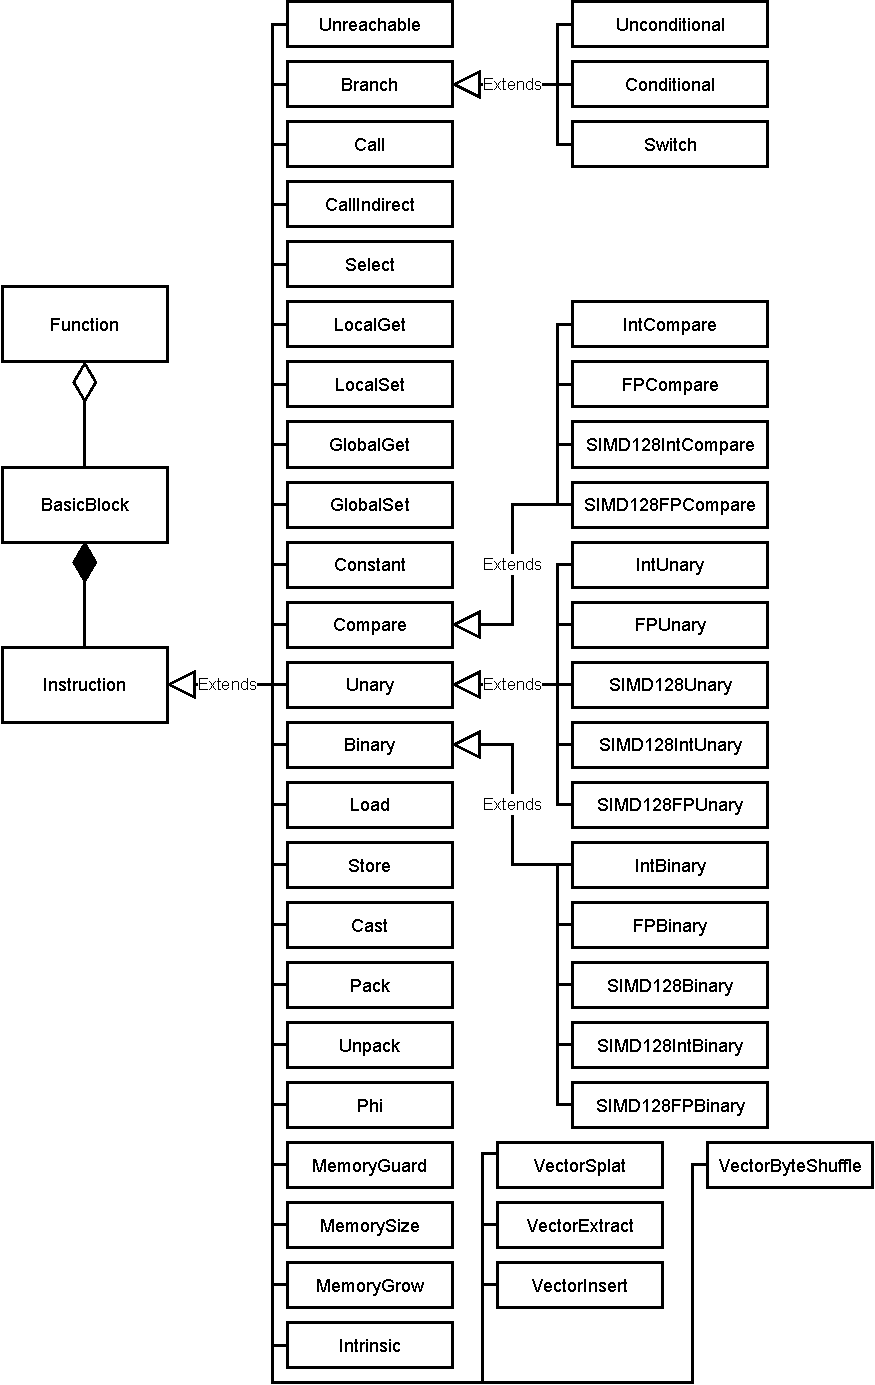
\includegraphics[width=0.8\textwidth]{Images/4.MIR/sablewasm-instruction.pdf}
  \caption{SableWasm MIR Instructions}
  \label{fig:sablewasm-mir-inst}
\end{figure}

\paragraph{Terminating instructions}
As discussed above, SableWasm splits the function control flow into basic
blocks containing the maximum number of consecutive instructions without
control flow transfer. In addition, SableWasm, similar to many other SSA form
instruction sets, defines a particular group of instructions called terminating
instructions. These instructions signal a control flow transfer out of the
current basic block, and they must only appear as the last instruction in any
given basic block. SableWasm defines four different terminating instructions:
unreachable, unconditional branching, conditional branching, and table
branching. If the control flow reaches a \texttt{Unreachable} instruction,
the runtime system will signal a runtime panic. The \texttt{Unreachable}
instruction in SableWasm is identical to its counterpart in WebAssembly in
terms of semantics. The \texttt{Unconditional} instruction is an unconditional
control flow transfer, as the name suggests. It refers to a target basic block
as the operand. At runtime, the instruction will always transfer the control
flow to the target basic block. \texttt{Unconditional} is similar to the
\texttt{br} instruction defined in WebAssembly specification. On the other hand,
\texttt{Conditional} is a conditional branching. It takes a value and two
target basic blocks as its operands. At runtime, the instruction will first
compare the value against integral value zero. If the value equals zero, the
instruction will transfer the control flow to the `false' basic block,
otherwise, to the `true' basic block. SableWasm's \texttt{Conditional}
instruction is similar to \texttt{br.cond} defined in WebAssembly. The last
terminating instruction defined in SableWasm is \texttt{Switch}.
\texttt{Switch} instruction is comparable to the \texttt{br.table} instruction
in WebAssembly. The instruction takes a value, a list of target basic blocks,
and a default branching basic block as its operands. At runtime,
\texttt{Switch} will interpret the value as an integral value and dispatch
accordingly. If the value is within the branching list's range, it will
redirect the control flow to the target basic block referred to by the index.
Otherwise, \texttt{Switch} will transfer the control flow to the default basic
block.

\paragraph{Function call}
In SableWasm, we provide two instructions for function calls defined in
WebAssembly specification: direct function calls and indirect function calls.
\texttt{Call} represents a direct function call where the callee is known at
compile time. It takes a function and a list of arguments as operands. On the
other hand, \texttt{CallIndirect} defines an indirect function call. It
implements the indirect function call protocol described in the WebAssembly
specification. A quick reminder, in WebAssembly, an indirect function call takes
an indirect table, the table index, the expecting function type, and a list of
values as arguments. At runtime, the system should first check if the index is
valid for the indirect table and fetch the function pointer and its actual
signature accordingly. Then, the system should compare the signature against the
expecting type. If the signature matches, the runtime system will
transfer the control flow to the function referred to by the function pointer.
Implementing the signature verification mechanism is backend-specific; we will
return to this topic in the next chapter. Note that we do not treat function
call instructions as terminating instructions, even though they transfer the
control flow to other locations. In SableWasm MIR, we follow the design like
that used in the LLVM intermediate representation, where it is assumed that
the control flow will continue to the next instruction after returning from the
function call. Hence, from the basic block's local perspective, their control
flow is pre-determined, and there is no difference compared to other
non-terminating instructions.

\paragraph{Local and global variable access}
In WebAssembly, instructions have access to locals defined by their parent
functions and global variables defined by their enclosing module. The SableWasm
MIR defines getter and setter instruction for both local and global variables to
implement the specification. Their semantics are the same compare to
WebAssembly's counterparts. We will skip the detail here, but one can consult
the WebAssembly specification for detailed information.

\paragraph{Numerical operations}
In SableWasm, we classify the numerical operations into three different
categories, the \texttt{Compare} instructions, \texttt{Unary} instructions, and
\texttt{Binary} instructions. The \texttt{Compare} instructions implement the
comparison between values, such as `equal to'. They always yield a 32-bit
integer as WebAssembly specification suggests. The \texttt{Unary} and
\texttt{Binary}, as their name suggests, perform unary and binary operations
between values. The result of \texttt{Unary} and \texttt{Binary} instruction is
dependent on the opcode. On the other hand, we can also orthogonally classify
the instructions into integer, floating-point, packed integer, and packed
floating-point numbers. Note that in MVP WebAssembly, there are only integer and
floating-point value operations; the SIMD operation extension proposal adds the
packed value operation to the instruction set. In the WebAssembly SIMD extension
proposal, the vector value does not store its size and content information in
the types. Instead, the packed value instructions' opcodes keep track of the
shape of the vector values, which leads to the bloated instruction opcodes. In
SableWasm, we separate the instruction opcode from the vector shape. For each of
the packed value operations, it must have either a \texttt{SIMD128IntLaneInfo}
or \texttt{SIMD128FPLaneInfo}. Figure~\ref{fig:sablewasm-mir-inst} shows all the
classes of numerical operations defined in SableWasm. For detailed opcodes in
each numerical instruction class, one can consult SableWasm's source code.

\paragraph{Load and Store}
\texttt{Load} and \texttt{Store} instruction provides access to the linear
memory for SableWasm MIR. Although in the current version of WebAssembly, the
module can contain at most one linear memory, and all WebAssembly's load and
store instructions implicitly refer to this linear memory \footnote{This might
  change in the future version of WebAssembly.}. In SableWasm MIR, we take a
different approach. The SableWasm MIR's \texttt{Load} instruction takes a linear
memory and an integer value as operands. At runtime, the value will be treated
as the address (or offset) to the start of the linear memory, and the
instruction yields the fetched result. In WebAssembly, the \texttt{load}
instruction associates with a type and an extension method. For example,
\texttt{i32.load8\_s} loads an 8-bit integer from the linear memory, and then
sign extends the fetched byte into a 32-bit integer. In SableWasm, the
\texttt{Load} instruction associates to a type and an integer value, namely the
load width. The load width must equal to or smaller than the width of the type.
Also, SableWasm \texttt{Load} always perform zero-extension on loaded value.
Hence, when translating WebAssembly's sign-extended load into SableWasm's
\texttt{Load}, one must combine the load instruction with a cast instruction.
We will come back to this in chapter~\ref{chapter:mir-translation-optimization}.
The \texttt{Store} instruction
also associate with a store width. Like the load width defined for \texttt{Load}
instruction, the store width must also be equal to smaller than the store value
type's width. The system will first bit truncate the value at runtime and then
store the result into the linear memory. One may notice that in SableWasm, we
erase the alignment attribute and offset attribute defined in WebAssembly.
Currently, we do not support alignment hints from the WebAssembly module. In
SableWasm, the \texttt{Load} and \texttt{Store} always have the alignment
requirement of one byte. This implies that the \texttt{Load} and \texttt{Store}
can happen anywhere in the linear memory, corresponding to WebAssembly's linear
memory specification.

\paragraph{Linear memory manipulation}
WebAssembly specification defines two instruction that works with linear
memories: \texttt{memory.size}, \texttt{memory.grow}. Like the WebAssembly's
\texttt{load} instruction we covered in the previous paragraph, all these
instructions operate over the implicitly defined unique linear memory within the
module. In SableWasm, we provide similar \texttt{MemoryGrow} and
\texttt{MemorySize} instruction. The semantics of SableWasm's memory
manipulation instructions are the same as their WebAssembly counterparts, except
that the linear memory needs to be explicitly stated. In SableWasm, we introduce
one additional instruction, \texttt{MemoryGuard} which is an explicit memory
boundary check. In WebAssembly, all \texttt{load} and \texttt{store} instruction
need to check for linear memory out of bound error before access. SableWasm
separates the bound check from the memory access. One advantage of this is that
one may implement static memory bounds check elimination optimization over
SableWasm MIR. Additionally, one backend may provide different strategies for
handling boundary checks, such as utilizing invalid virtual memory pages with
the operating system's help. In this case, we only need to modify the
translation pattern for \texttt{MemoryGuard}. \texttt{MemoryGuard} takes a
linear memory and an integer value as the operand. It also associates with an
integer immediate, known as the guard width. At runtime, the system will perform
a boundary check over the linear memory starting from the given address to
determine if it contains at least a given number of bytes ahead. If there are
not enough bytes available, the system should signal a runtime panic.

\paragraph{Pack and Unpack}
WebAssembly multivalue specification \footnote{WebAssembly Multi-value Proposal:
  \url{https://github.com/WebAssembly/multi-value}} relaxes the constrains on
the function type. Functions now can return multiple values instead of at most
one value. To support these features, we introduce \texttt{Pack} and
\texttt{Unpack} instructions, along with extending WebAssembly's type system.
\texttt{Pack} instructions group multiple values into a single ordered tuple,
while the \texttt{Unpack} reverse the operation by retrieving the value from
tuples by index. In the case where a function returns multiple values, we thus
use a tuple instead. SableWasm treats tuples as first-class values; however,
currently, tuples cannot be recursive. We will come back to this
in chapter~\ref{chapter:mir-translation-optimization},
when we visit the type systems of SableWasm MIR. The index of the
\texttt{Unpack} must be an immediate value in the current version of SableWasm
MIR and is verified at compile time.

\paragraph{Vector operations}
In the previous paragraph, we introduce the numeric operations defined in
SableWasm MIR. However, several instructions do not fit into either
\texttt{Unary} or \texttt{Binary} instructions. Hence, to faithfully support the
SIMD operations introduced by the extension proposal, we add four
vector-specific operations into SableWasm MIR. They are \texttt{VectorSplat},
\texttt{VectorExtract}, \texttt{VectorInsert} and \texttt{VectorByteShuffle}.
\texttt{VectorSplat} will broadcast the operand value to all lanes in the result
vector. SableWasm MIR defines vector splat operation for both packed integer
vector and packed floating-point vector. \texttt{VectorExtract} is similar to
the \texttt{extractelement} defined in LLVM intermediate representation. It
takes a vector as the operand and also associates itself with an immediate
integer value. At runtime, the system extracts the value of the given lane and
yields as a result. \texttt{VectorInsert} is similar to \texttt{insertelement}
defined in LLVM. It will replace the vector operand with a given value and
yields the updated vector as a result. Note that in the WebAssembly SIMD
extension proposal, there are more instructions defined that modify the
individual lane value of the vector, such as \texttt{V128Load32Lane} which
loads a 32-bit value into a specific lane within the vector. In this project,
we would like to keep our instruction set simple; hence, these instructions are
reduced into multiple SableWasm MIR instructions. We will come back to this
in chapter~\ref{chapter:mir-translation-optimization}
when we discuss the instruction reduction rules. The last
instruction we introduced is the \texttt{VectorByteShuffle}.
\texttt{VectorByteShuffle} is similar to \texttt{shufflevector} defined in LLVM,
except that it allows rearranging bytes instead of lanes. Currently, the
\texttt{VectorByteShuffle} only operates over an array of immediate integer
values. Compare to the lane shuffle semantics, byte shuffle semantics provides
more precise control over the result value. One can trivially simulate a lane
shuffle with a byte shuffle. The WebAssembly SIMD extension proposal only
defines shuffle for \texttt{i8x16}, which corresponding to the byte shuffle
semantics. However, in the future, if another shape vector supports shuffle
operation, one can generalize the implementation with minimal modification.

\paragraph{Cast}
\texttt{Cast} models the conversion of values to their equivalent form in other
types. In SableWasm MIR, we do not distinguish between value conversion and
value extension. We treat signed and zero extensions as a kind of value
conversion. The \texttt{Cast} instruction takes a single value as the operand,
and it associates itself with a cast opcode. At runtime, it will perform the
conversion according to the opcode, and if the result cannot be accurately
represented in the target type, the system should signal a runtime error.
The cast opcodes are direct implementations of their WebAssembly counterparts,
and we will skip the detail here. One may refer to the WebAssembly specification
for more details.

\paragraph{Intrinsic}
The last SableWasm MIR instruction we are going to cover in this section is the
\texttt{Intrinsic} instructions. Most WebAssembly instructions can be
represented by using the SableWasm MIR instructions, which we covered earlier in
this section. However, there are still several corner cases. For example, the
WebAssembly SIMD extension proposal defines Q-format rounding multiplication, a
type of fix-point multiplication, for packed 16-bit integers. Another example is
the \texttt{swizzle} operation. A \texttt{swizzle} operation is similar to a
shuffle operation, except that it takes another vector as the shuffle indices
vector instead of an array of immediate integer values. These operations are
only defined for a specific vector shape and will introduce unneeded complexity
to the SableWasm MIR if we generalize them to all possible vector shapes. Hence,
here we group these instructions as the \texttt{Intrinsic} instructions. There
is no direct mapping to LLVM instruction for most of them, even with the
intrinsic functions provided by the framework. Hence, the backend is encouraged
to support these instructions with runtime library routines.

In this section, we discussed the design of the SableWasm MIR instruction set,
and in the next chapter, we will move to the translation strategy between
WebAssembly and SableWasm MIR along with the analysis and transformation
framework.

\section{Translating WebAssembly to MIR}

In this section, we will cover the translation between WebAssembly bytecode and SableWasm MIR. We have covered the design of SableWasm MIR instructions previously. One may notice that for most of the instructions, especially for the numerical operations, SableWasm MIR shares the same semantics as WebAssembly. Hence, the translation rules for these instructions are pretty trivial, and we will not cover them in detail in this section. Instead, this section will focus on the translation rules for the structured control flow construct and WebAssembly instructions that require reduction during translation.

The translation framework is similar to the validation framework we discussed in the previous chapter except for two significant differences. First, the operation stack will keep track of the values generated during translation instead of types. Let's take \texttt{i32.add} as an example. \texttt{i32.add} instruction takes two values from the stack and then performs 32-bit integer addition between them. Finally, it will push the result type back onto the stack. In the case of translation stack, we pop two values from the stack and assume they are 32-bit integers. In SableWasm MIR, we use pointers to instructions to refer to the values generated by them. Then, the translation visitor will build a \texttt{IntBinaryOp} instruction, with \texttt{Add} as opcode, and two pointers as operands. Finally, the visitor will append the instruction to the current active basic block and push the instruction pointer of \texttt{IntBinaryOp} onto the stack. Another difference between the validation framework and the translation framework is the labels stack. In the validation framework, the labels stack stores the resulting types generated from the label. In the translation framework, the labels stack stores the potential landing basic blocks for the labels. We will revisit this with more details later in this section.

\subsection{Structured-Control-Flow Construct}

Translating from stack-based IR to register-based IR is not trivial, especially
when non-linear control flow structures appeared. This problem appeared in many
runtime system implementations, such as Numba \cite{numba}, a just-in-time (JIT)
compiler for Python. Usually, one needs some algorithm to recover the control
flow structure from annoying jump instructions. Luckily, in WebAssembly, we can
translate the stack-based bytecode into register-based basic blocks in linear
time, thanks to the structured control flow constructs and their validation
rules defined in WebAssembly. In this section, we will cover the translation
patterns used for WebAssembly's structured-control-flow constructs, namely
\texttt{block}, \texttt{if} and \texttt{loop}.

\begin{figure}
  \centering
  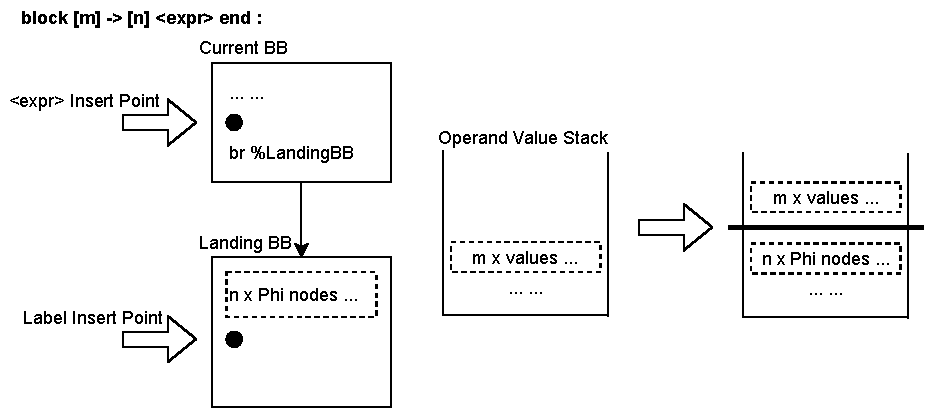
\includegraphics[width=\textwidth]{Images/4.MIR/translate-block.pdf}
  \caption{WebAssembly \texttt{block} translation pattern}
  \label{fig:translate-block}
\end{figure}

\begin{figure}
  \centering
  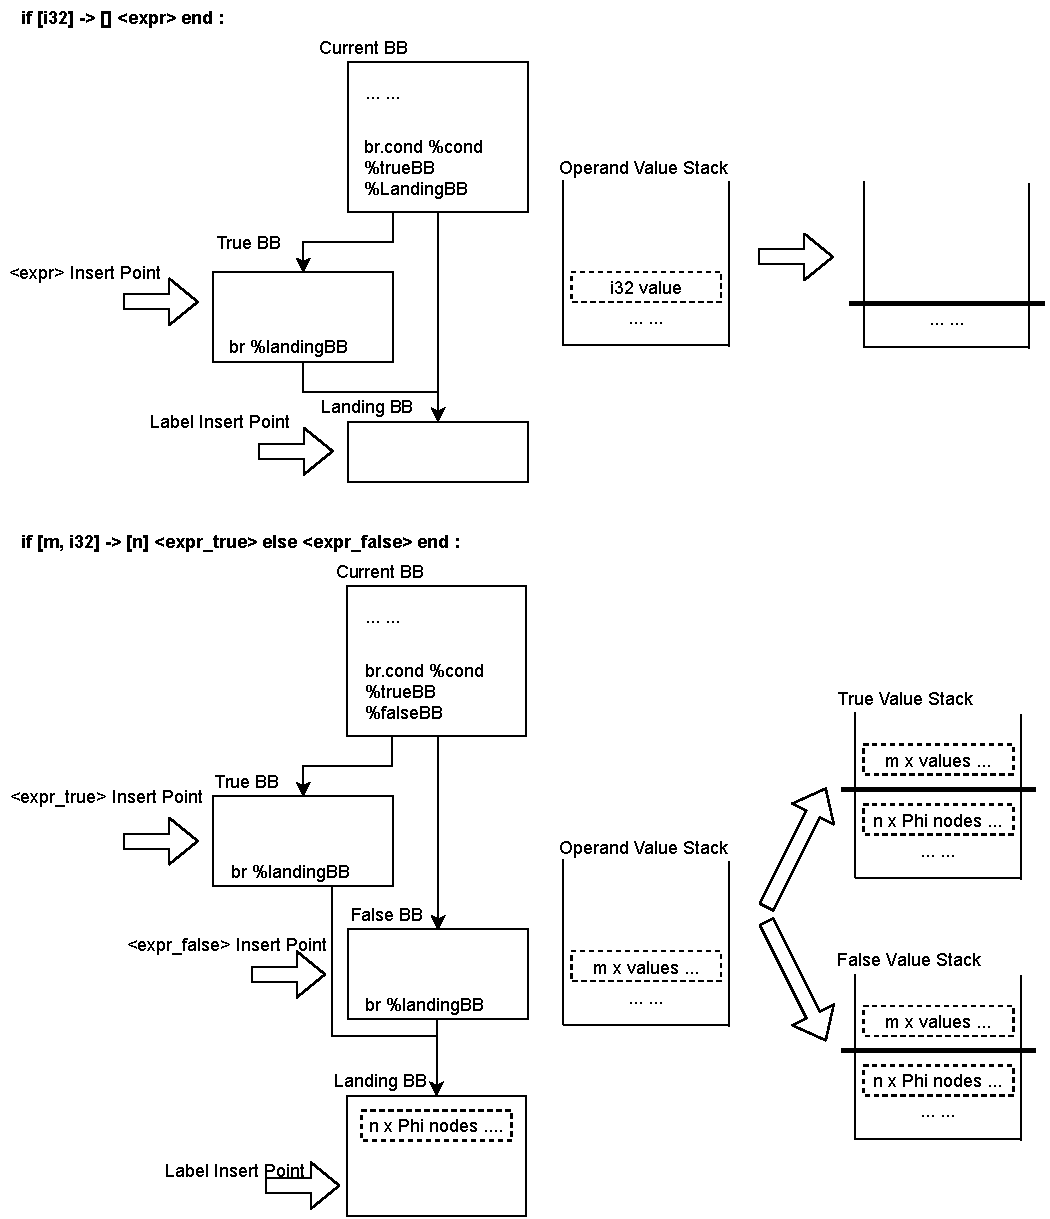
\includegraphics[width=\textwidth]{Images/4.MIR/translate-if.pdf}
  \caption{WebAssembly \texttt{if} translation pattern}
  \label{fig:translate-if}
\end{figure}

\paragraph{Block}
In the background chapter, we provide a general illustration of the three
structured control flow constructs. As a quick recap, \texttt{block} is the
simplest form of a structured control flow construct. It implicitly introduces
a label at the end of its enclosing instructions. A branch instruction
referring to this label will redirect the control flow to the end of the block.
Figure~\ref{fig:translate-block} illustrates the translation pattern for
WebAssembly \texttt{block} in SableWasm MIR. We will first clarify some of the
terminologies we used in the figure, and we will use the same terms later in
the \texttt{loop} and \texttt{if} pattern discussion for consistency.
\emph{Expr Insert Point} refer to the starting position for the generated
instructions when we recursively translate the instructions within the enclosing
expression of the \texttt{block} instruction. Furthermore,
\emph{Label Insert Point} refer to the position for generated instructions when
we finish the recursive translation and resume to the parent expression of the
\texttt{block} instruction. A \emph{label stack entry} is a tuple consisting of
a pointer to the landing basic block, a list of $\phi$ nodes expecting merge
values, and a pointer to the \emph{label insert point}. The translation pattern
for \texttt{block} is pretty simple; we continue on the current basic block and
prepare the landing basic block for the block instruction as a branch
instruction within the expression may refer to the label. Additionally, to fully
support multi-value extension in WebAssembly, we also need to prepare the $\phi$
nodes in the landing basic block. SableWasm generates the $\phi$ nodes based on
the type of the \texttt{block} instruction. WebAssembly validation rules ensure
that the expression within the \texttt{block} can access exactly $m$ values from
the stack and put $n$ values onto the stack. Finally, we will append an
unconditional branch to the landing basic block because in WebAssembly,
if the control flow reaches the bottom of the \texttt{block} expressions, it
will implicitly fall through. For the operand stack, we will first pop $m$
values from the stack as \texttt{block} instruction's type suggests and push the
$\phi$ nodes as the result values. Then, we need to set up the boundary between
the operand stack for the expression contained within the \texttt{block}.
Figure~\ref{fig:translate-block} represents this with the bold line in the
result operand value stack. The last step is to push the $m$ values back to the
stack, as they are passed to the expression within the \texttt{block}.


\paragraph{If}
The next control-flow structure defined WebAssembly is \texttt{if}.
WebAssembly's \texttt{if} is an expression instead of a statement that appears
in many other languages such as C. The \texttt{if} expression can yield some
values indicated by its type. Figure~\ref{fig:translate-if} illustrates the
translation patterns in SableWasm. There are two types of \texttt{if}
instruction defined in WebAssembly specification. The first case is a `partial'
\texttt{if} instruction, where it only contains the `true' branch. From
WebAssembly validation rules, it's easy to show that the only possible type is
\texttt{[i32]->[]}, even with the multi-value extension proposal. This implies
that the expression within the \texttt{if} instruction must start with an empty
operand stack. Hence, the translation pattern for the partial \texttt{if} is
quite straightforward: we only need to pop the condition value from the operand
stack and construct a conditional branch based on this value in the current
basic block. On the other hand, we also have `full' \texttt{if} instructions
with both `true' and `false' expressions. The validation rules ensure that both
expressions must have the same type. The translation pattern is more complex
compare to that of a `partial' \texttt{if}. In this case, we have to prepare the
landing basic block similar to what we did for the \texttt{block} construct.
We need to generate $n$ $\phi$ nodes for data-flow mergers from the `true'
branch, the `false' branch, and any possible branch instruction within both
nested expressions. Similarly, we need to pop $m$ values from the stack for
operand values stack and then push $n$ $\phi$ nodes. And, within both nested
expressions, push $m$ values back to the stack.

\begin{figure}
  \centering
  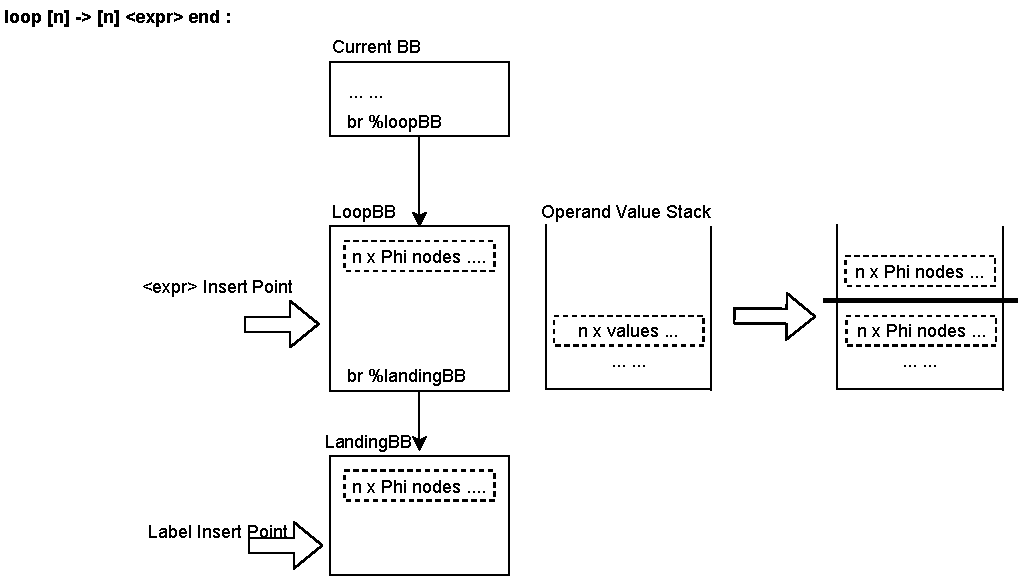
\includegraphics[width=\textwidth]{Images/4.MIR/translate-loop.pdf}
  \caption{WebAssembly \texttt{loop} translation pattern}
  \label{fig:translate-loop}
\end{figure}

\paragraph{Loop}
The last control-flow structure defined in WebAssembly is \texttt{loop}.
Figure~\ref{fig:translate-loop} gives a general illustration of SableWasm's
translation pattern for \texttt{loop} instructions. Similar to the `partial'
\texttt{if} we discussed in the previous paragraph, one can show that, under
WebAssembly's validation rules, the parameter types for the \texttt{loop}
instruction must equal to the result types. The \texttt{loop} instruction is
similar to the \texttt{block} instruction, except that if any branch
instruction refers to it, the branch instruction should transfer the control
flow to the start of the expression within the instruction instead of the end.
Thus, we need to prepare a standalone basic block for the nested expression in
\texttt{loop}, along with the $\phi$ nodes to merge value on each loop
iteration. Note that we also introduce $\phi$ nodes in the landing basic block.
One may argue that there is no need for these $\phi$ nodes, as only one block
can reach the loop exit, and no value merging will occur. Indeed, these
$\phi$ nodes will always be trivial $\phi$ nodes, which have only one
possible value inflow. However, this is due to the limitation of our translation
framework.

In this section, we discussed the translation patterns for WebAssembly
structured control flow constructs. Thanks to WebAssembly validation rules, the
types for these structured control flow instructions explicitly mark value
merging and imply possible $\phi$ nodes. Furthermore, one can show that the
control graph generated above is indeed in SSA form. However, the directly
generated control flow graph is not easily understandable by users. This mainly
comes from two facts. First, the WebAssembly-targeting compiler may generate
awkward patterns to fit in the structured control-flow constructs. Second,
SableWasm translation patterns for structured-control flow constructs are not
optimal.
\subsection{Instructions Reduction}

This section will cover the instructions reduction rules used when lowering WebAssembly bytecode to SableWasm MIR. In the background chapter, we mentioned that one of WebAssembly's design goals is to be as compact as possible. When the community design the WebAssembly instruction set, they fuse several typical instruction sequences into single instructions. For example, SIMD vector operation extension defines \texttt{v128.load8x8\_s} which first load 8 single-byte integers into a vector, and then sign-extended them into 16 bit integers. Another example will be \texttt{v128.load32\_lane} which loads a 32-bit value, either a 32-bit integer or a single-precision floating-point number into a given vector. Such design is understandable for WebAssembly as binary size do matter when shipping application over the internet. But, for SableWasm, a static compiler, we focus more on the size of the instruction set instead of the size of the intermediate representation. It is harder to write analysis for a bloated instruction set, as one needs to consider more instruction cases. Hence, when lowering WebAssembly bytecode to SableWasm MIR, we replace some WebAssembly instructions with a sequence of SableWasm MIR instructions.


\paragraph{Eqz} \quad
\begin{lstlisting}[basicstyle=\linespread{1}\small, language=LLVM]
[..., %n i32] i32.eqz => %t0 = i32.const 0; %t1 = int.eq %n %t0
[..., %n i64] i64.eqz => %t0 = i64.const 0; %t1 = int.eq %n %t0
\end{lstlisting}
WebAssembly defines unary \texttt{eqz} operations for all integer values. As the name suggests, \texttt{eqz} compares the operand value against zero and yields to one if true, zero otherwise. In SableWasm MIR, we group all comparison instructions into \texttt{Compare} class, and \texttt{eqz} does not fit into the class as it is not a binary operation. Hence we rewrite the \texttt{eqz} as \texttt{Compare} instruction with opcode as \texttt{Eq}.

\paragraph{Load} \quad
\begin{lstlisting}[basicstyle=\linespread{1}\small, language=LLVM]
[..., %base i32] i32.load offset=%offset align=%align =>
    %addr = int.add %base %offset;
    memory.guard %mem %addr 4;
    %t0 = load.32 i32 %mem %addr
[..., %base i32] i32.load16_u offset=%offset align=%align =>
    %addr = int.add %base %offset;
    memory.guard %mem %addr 2;
    %t0 = load.16 i32 %mem %addr
[..., %base i32] i32.load16_s offset=%offset align=%align =>
    %addr = int.add %base %offset;
    memory.guard %mem %addr 2;
    %t0 = load.16 i32 %mem %addr;
    %t1 = cast i32.extend.16.s %t0
\end{lstlisting}



\section{Analysis Framework}
\begin{figure}
  \centering
  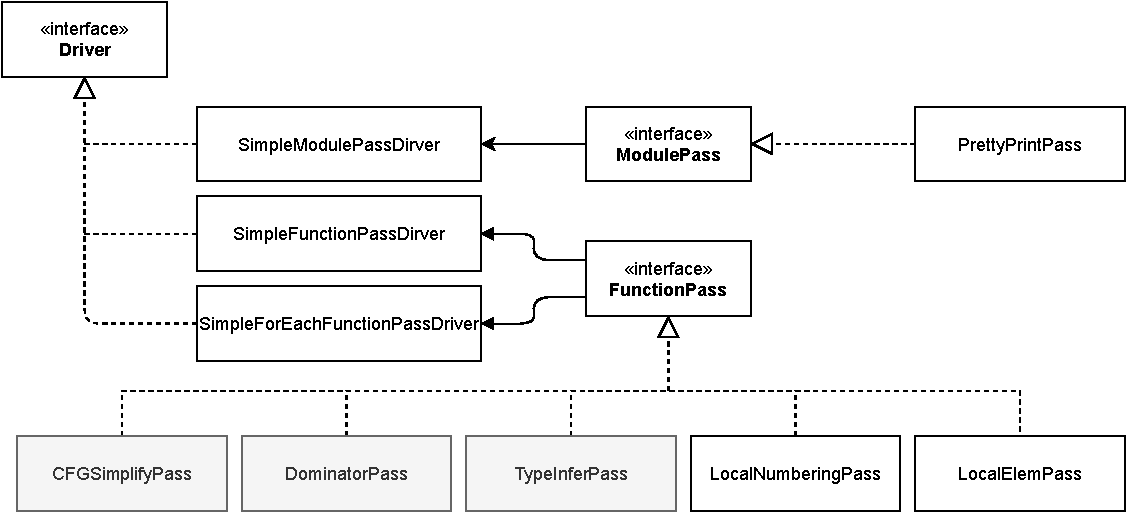
\includegraphics[width=\textwidth]{Images/4.MIR/analysis-framework.pdf}
  \caption{SableWasm MIR Analysis and Optimization Framework}
  \label{fig:sablewasm-mir-analysis-framework}
\end{figure}
SableWasm also implements an analysis and optimization framework over middle-level intermediate representation (MIR). The framework consists of two parts, passes and drivers. SableWasm analysis and transformation framework only provides essential support for managing passes, compared to other more advanced frameworks, such as McSAF\cite{mcsaf}, an optimization framework for MATLAB language. Figure~\ref{fig:sablewasm-mir-analysis-framework} illustrates the current state of the framework in SableWasm. Currently, we implement three different drivers. \texttt{SimpleModulePassDirver} accepts module passes and operates on the module level. At the time of thesis writing, we haven't explored the inter-procedure analysis for SableWasm MIR in detail, and the only module pass implemented is the pretty print pass.

\subsection{Control-Flow Graph Simplification}

\subsection{Dominators and Dependence}

\subsection{Type Infer}

\subsection{Local Value Numbering}

\subsection{Redundant Local Variable Elimination}